\documentclass[12pt,a4paper]{article}

\usepackage[utf8]{inputenc}
\usepackage[T1]{fontenc}
\usepackage[italian]{babel}
\usepackage{geometry}
\usepackage{graphicx}
\usepackage{float}
\usepackage{array}
\usepackage{longtable}
\usepackage{tabularx}
\usepackage{enumitem}
\usepackage{xcolor}
\usepackage{hyperref}
\usepackage{titlesec}
\usepackage{fancyhdr}
\usepackage{lastpage}
\usepackage{booktabs}

\geometry{margin=2.5cm}
\hypersetup{
    colorlinks=true,
    linkcolor=black,
    urlcolor=blue,
    pdftitle={BugBoard26 - Specifica e verifica dei requisiti},
    pdfauthor={Gruppo BugBoard26}
}

\definecolor{sectionblue}{RGB}{24,68,112}
\definecolor{lightgray}{RGB}{245,245,245}
\definecolor{tablehead}{RGB}{230,238,247}

\titleformat{\section}{\Large\bfseries\color{sectionblue}}{\thesection}{1em}{}
\titleformat{\subsection}{\large\bfseries\color{sectionblue}}{\thesubsection}{1em}{}
\titleformat{\subsubsection}{\normalsize\bfseries\color{sectionblue}}{\thesubsubsection}{1em}{}

\pagestyle{fancy}
\fancyhf{}
\lhead{BugBoard26}
\rhead{Specifica e verifica dei requisiti}
\cfoot{Pagina \thepage\ di \pageref{LastPage}}

\setlength{\parindent}{0pt}
\setlength{\parskip}{0.6em}
\renewcommand{\arraystretch}{1.25}

\newcommand{\placeholder}[2]{%
\begin{figure}[H]
\centering
\fbox{%
\begin{minipage}[c][#2][c]{0.88\textwidth}
\centering
\textit{#1}
\end{minipage}}
\end{figure}
}

\begin{document}

\begin{titlepage}
    \centering
    \vspace*{2cm}
    {\Huge \textbf{BugBoard26} \par}
    \vspace{0.5cm}
    {\Large Specifica e verifica dei requisiti \par}
    \vspace{1cm}
    {\large Progetto di Ingegneria del Software \par}
    {\large A.A. 2025/2026 \par}
    \vfill
    \begin{tabular}{ll}
        \textbf{Componenti:} & Valerio Porcile - N86004517 \\
                              & Emanuel Giuseppe Lupoli - N86004280 \\
                              & Emanuele Martucci - N86004084 \\
        \textbf{Modalita':} & Tradizionale \\
        \textbf{Versione documento:} & 0.1 \\
        \textbf{Data:} & \today \\
    \end{tabular}
    \vfill
\end{titlepage}

\tableofcontents
\newpage

\section{Introduzione}

Il presente documento descrive i requisiti individuati per il sistema \textbf{BugBoard26}, una piattaforma per la gestione collaborativa di issue relative a progetti software. Il sistema consente agli utenti autenticati di segnalare problemi o richieste, consultarli, cercarli, filtrarli e seguirne l'evoluzione fino alla risoluzione.

Il documento è stato prodotto a partire dalla traccia del progetto e dalle funzionalità assegnate al gruppo. Le funzionalità non assegnate non sono state incluse, salvo piccoli elementi tecnici necessari per rendere coerente il sistema. Ad esempio, viene previsto un assegnatario per le issue perché alcune funzionalità richieste dipendono da questo concetto.

\subsection{Scopo del documento}

Lo scopo del documento è definire in modo chiaro:

\begin{itemize}[noitemsep]
    \item gli attori che interagiscono con il sistema;
    \item i requisiti funzionali e non funzionali;
    \item i casi d'uso principali;
    \item i criteri di verifica usati per controllare che i requisiti siano stati soddisfatti;
    \item i primi mock-up delle schermate previste.
\end{itemize}

\subsection{Funzionalità assegnate}

Le funzionalità assegnate al gruppo sono le seguenti:

\begin{center}
\begin{tabularx}{\textwidth}{>{\bfseries}c X}
\toprule
N. & Funzionalità \\
\midrule
1 & Autenticazione tramite email e password, con account amministratore iniziale e creazione utenti da parte dell'amministratore. \\
2 & Creazione di issue da parte degli utenti che hanno effettuato l'accesso, con titolo, descrizione, tipo, priorità opzionale e immagine opzionale. \\
3 & Vista riepilogativa delle issue, con filtri e ordinamento. \\
6 & Cambio di stato da parte dell'utente assegnato e notifica al segnalatore quando la issue viene risolta. \\
8 & Esportazione dell'elenco delle issue in un formato condivisibile. \\
11 & Ricerca delle issue tramite parole chiave. \\
13 & Archiviazione delle issue da parte degli amministratori e consultazione delle issue archiviate. \\
14 & Suggerimento automatico dell'assegnatario in base al carico di lavoro corrente. \\
15 & Modalità readonly per utenti esterni, con sola consultazione delle issue. \\
16 & Contrassegno di una issue come duplicata e chiusura immediata. \\
\bottomrule
\end{tabularx}
\end{center}

\section{Glossario}

\begin{longtable}{>{\bfseries}p{0.25\textwidth} p{0.68\textwidth}}
\toprule
Termine & Descrizione \\
\midrule
Issue & Segnalazione inserita nel sistema. Può rappresentare un bug, una domanda, un problema di documentazione o una richiesta di funzionalità. \\
Utente autenticato & Utente che ha effettuato il login e possiede un ruolo nel sistema. \\
Utente normale & Utente che può creare issue, consultarle e modificare lo stato delle issue assegnate a lui. \\
Amministratore & Utente con privilegi aggiuntivi, tra cui creazione utenti, archiviazione, export e gestione dei duplicati. \\
Utente readonly & Utente esterno che può visualizzare le issue e i relativi dettagli, senza modificarli. \\
Assegnatario & Utente a cui è stata assegnata una issue. \\
Segnalatore & Utente che ha creato la issue. \\
Issue archiviata & Issue non più visibile nelle liste principali, ma ancora consultabile in una sezione dedicata. \\
Issue duplicata & Issue marcata come copia di un'altra già presente nel sistema. \\
Notifica & Messaggio interno al sistema usato per comunicare eventi rilevanti agli utenti. \\
\bottomrule
\end{longtable}

\section{Attori del sistema}

\begin{center}
\begin{tabularx}{\textwidth}{>{\bfseries}p{0.25\textwidth} X}
\toprule
Attore & Descrizione \\
\midrule
Utente autenticato & Attore generale che rappresenta qualsiasi utente che ha effettuato l'accesso al sistema. \\
Utente normale & Può creare issue, consultare le issue presenti, usare ricerca e filtri e cambiare lo stato delle issue assegnate a lui. \\
Amministratore & Gestisce utenti e funzioni amministrative, come archiviazione, export, duplicati e suggerimento dell'assegnatario. \\
Utente readonly & Può consultare le issue, cercarle e filtrarle, ma non può effettuare operazioni di modifica. \\
\bottomrule
\end{tabularx}
\end{center}

\clearpage
\section{Requisiti funzionali}

\begin{longtable}{>{\bfseries}p{0.12\textwidth} p{0.58\textwidth} p{0.18\textwidth}}
\toprule
ID & Descrizione & Priorità \\
\midrule
RF-01 & Il sistema deve permettere il login tramite email e password. & Alta \\
RF-02 & Il sistema deve prevedere un account amministratore iniziale. & Alta \\
RF-03 & Un amministratore deve poter creare nuovi utenti specificandone email, password e ruolo. & Alta \\
RF-04 & Un utente autenticato non readonly deve poter creare una issue indicando almeno titolo e descrizione. & Alta \\
RF-05 & Una issue deve poter avere tipo, priorità opzionale e immagine opzionale. & Media \\
RF-06 & Le issue appena create devono partire nello stato \textit{TODO}. & Alta \\
RF-07 & Il sistema deve mostrare una lista riepilogativa delle issue non archiviate. & Alta \\
RF-08 & Il sistema deve consentire filtro e ordinamento delle issue per criteri rilevanti, come tipo, stato e priorità. & Alta \\
RF-09 & Il sistema deve consentire la ricerca delle issue tramite parole chiave su titolo e descrizione. & Alta \\
RF-10 & L'utente assegnato a una issue deve poterne modificare lo stato. & Alta \\
RF-11 & Quando una issue passa allo stato \textit{RESOLVED}, il sistema deve notificare l'utente che l'ha segnalata. & Alta \\
RF-12 & Il sistema deve consentire l'esportazione dell'elenco delle issue in formato CSV. & Media \\
RF-13 & Un amministratore deve poter archiviare una issue. & Alta \\
RF-14 & Le issue archiviate non devono comparire nella lista principale. & Alta \\
RF-15 & Le issue archiviate devono essere consultabili in una sezione dedicata. & Media \\
RF-16 & Il sistema deve suggerire un assegnatario in base al carico di lavoro corrente degli utenti. & Alta \\
RF-17 & Un utente readonly deve poter visualizzare issue e dettagli senza modificare dati. & Alta \\
RF-18 & Un amministratore deve poter contrassegnare una issue come duplicata di un'altra. & Alta \\
RF-19 & Quando una issue viene marcata come duplicata, il sistema deve chiuderla immediatamente. & Alta \\
\bottomrule
\end{longtable}

\clearpage
\section{Requisiti non funzionali}

\begin{longtable}{>{\bfseries}p{0.12\textwidth} p{0.70\textwidth} p{0.12\textwidth}}
\toprule
ID & Descrizione & Categoria \\
\midrule
RNF-01 & Le password degli utenti non devono essere salvate in chiaro, ma memorizzate usando un algoritmo di hashing sicuro. & Sicurezza \\
RNF-02 & Le API devono verificare il ruolo dell'utente prima di eseguire operazioni riservate agli amministratori o agli utenti assegnati. & Sicurezza \\
RNF-03 & Frontend e backend devono essere separati e comunicare solo tramite API REST. & Architettura \\
RNF-04 & Lo stato persistente del sistema deve essere conservato nel backend e nel database, non nel frontend. & Architettura \\
RNF-05 & L'interfaccia deve essere semplice da usare durante la demo e deve rendere chiare le operazioni disponibili per ogni ruolo. & Usabilita' \\
RNF-06 & La lista issue deve restare consultabile in modo fluido per un numero ragionevole di segnalazioni inserite a scopo dimostrativo. & Prestazioni \\
RNF-07 & Il codice backend deve essere organizzato in modo da separare controller, servizi, modelli e accesso ai dati. & Manutenibilità \\
RNF-08 & Il progetto deve essere eseguibile in locale seguendo le istruzioni presenti nel README principale. & Deploy \\
\bottomrule
\end{longtable}

\clearpage
\section{Use Case Diagram}

Il diagramma dei casi d'uso riassume le interazioni principali tra gli attori e il sistema. Gli attori specializzati ereditano dall'attore generale \textit{Utente autenticato}, mentre le funzioni amministrative sono riservate all'amministratore.

\IfFileExists{UCD/use_case_diagram.png}{
\begin{figure}[H]
    \centering
    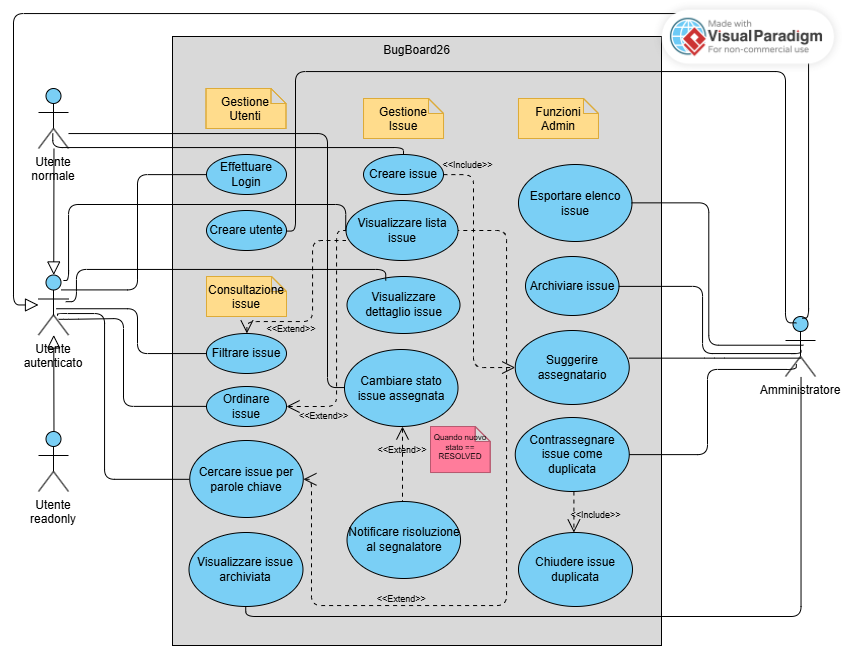
\includegraphics[width=0.95\textwidth]{UCD/use_case_diagram.png}
    \caption{Use Case Diagram di BugBoard26}
    \label{fig:use-case-diagram}
\end{figure}
}{
\begin{center}
    \fbox{\parbox{0.85\textwidth}{
        \centering
        Il file \texttt{UCD/use\_case\_diagram.png} non è stato trovato.
    }}
\end{center}
}

\clearpage
\section{Descrizione dei casi d'uso principali}

\subsection{UC-01 - Creare una issue}

\begin{tabularx}{\textwidth}{>{\bfseries}p{0.28\textwidth} X}
\toprule
Campo & Descrizione \\
\midrule
Attore primario & Utente normale \\
Scopo & Inserire una nuova segnalazione nel sistema. \\
Precondizioni & L'utente ha effettuato il login e non ha ruolo readonly. \\
Postcondizioni & La issue viene salvata nello stato \textit{TODO} ed è visibile nella lista principale. \\
Scenario principale &
\begin{enumerate}[noitemsep]
    \item L'utente apre la pagina di creazione issue.
    \item Il sistema mostra il form di inserimento.
    \item L'utente inserisce titolo, descrizione, tipo e, se necessario, priorità e immagine.
    \item Il sistema valida i dati inseriti.
    \item Il sistema salva la issue con stato iniziale \textit{TODO}.
    \item Il sistema mostra la nuova issue nella lista principale.
\end{enumerate} \\
Estensioni & Se titolo o descrizione sono mancanti, il sistema segnala l'errore e non salva la issue. \\
Requisiti collegati & RF-04, RF-05, RF-06, RF-07 \\
\bottomrule
\end{tabularx}

\IfFileExists{mock-up/Creazione issue.png}{
\begin{figure}[H]
    \centering
    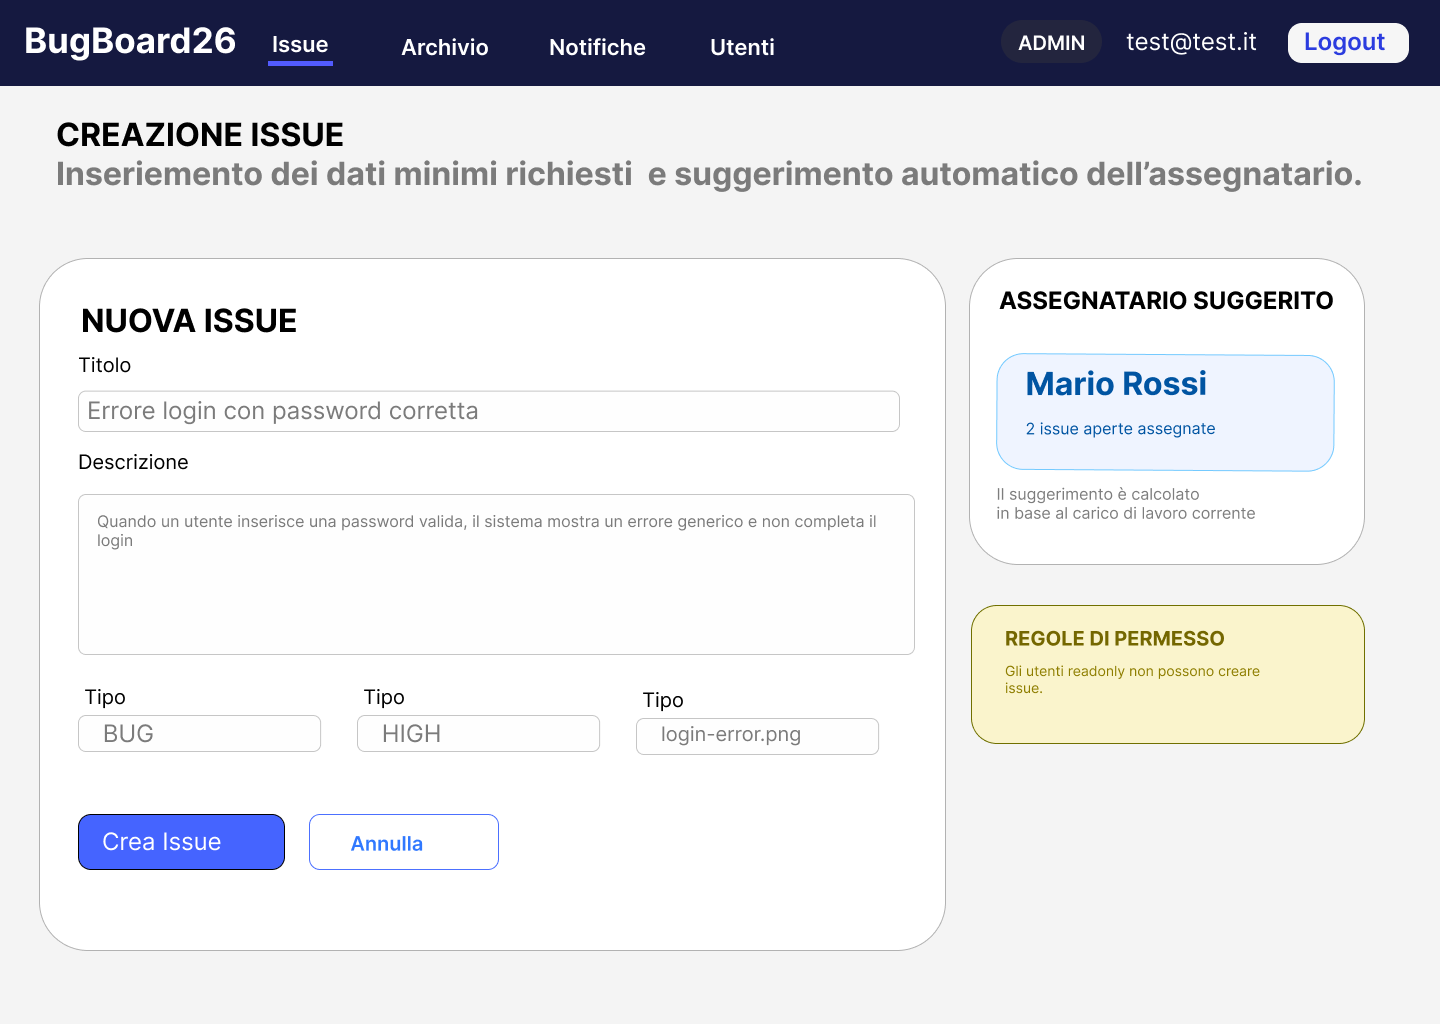
\includegraphics[width=0.9\textwidth]{mock-up/Creazione issue.png}
    \caption{Mock-up - Creazione issue}
\end{figure}
}{
\begin{figure}
    \centering
    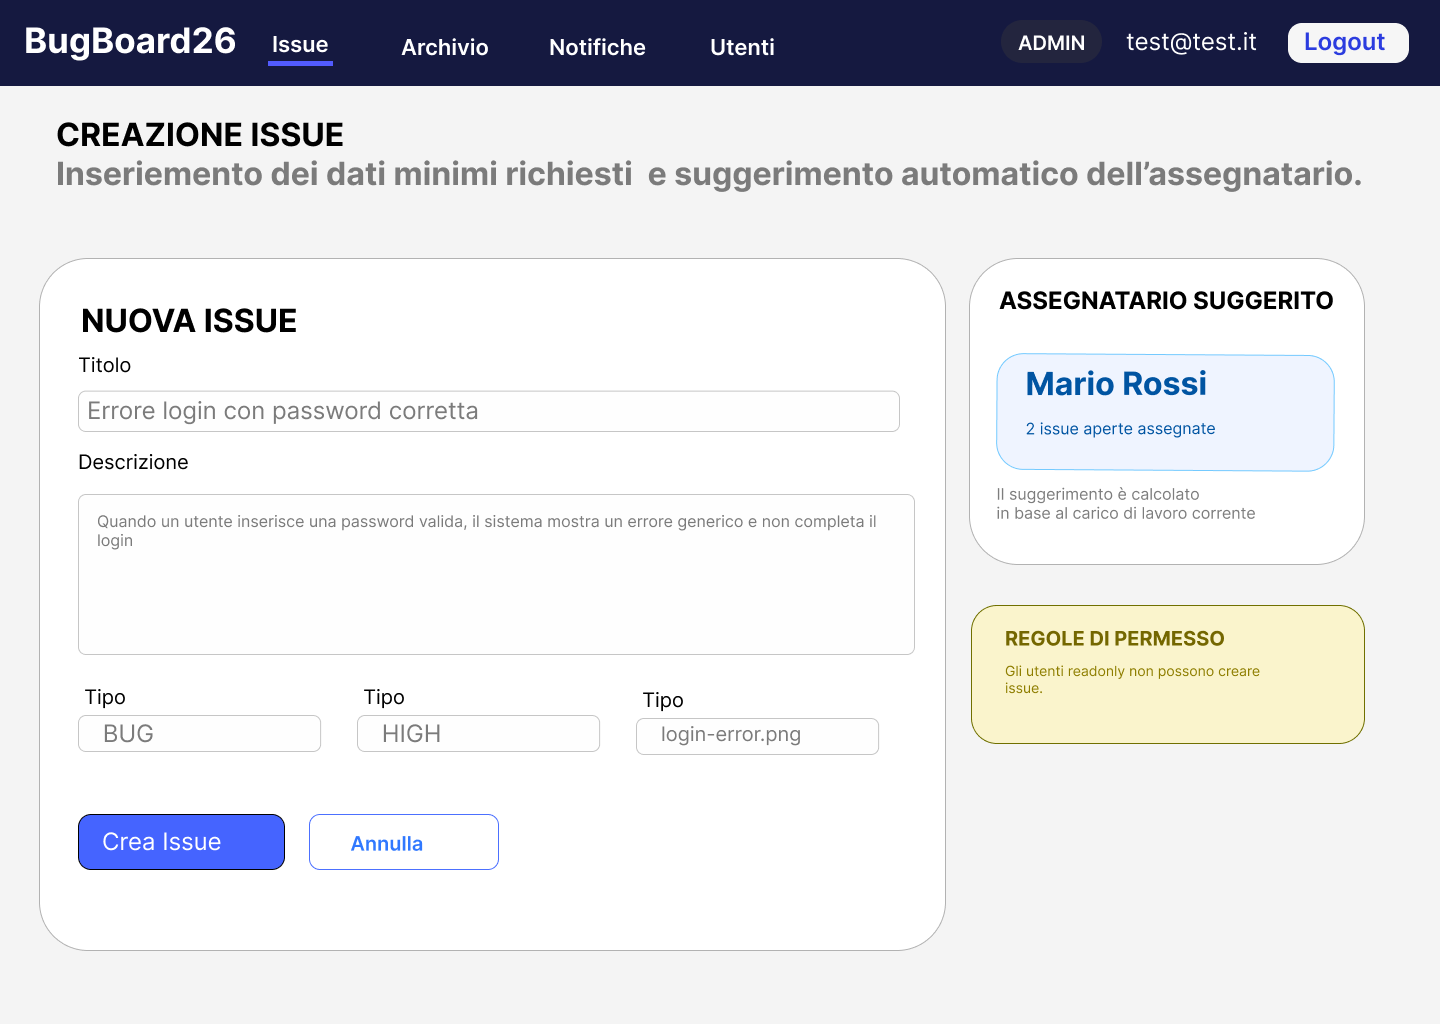
\includegraphics[width=0.5\linewidth]{mock-up/Creazione issue.png}
    \caption{Enter Caption}
    \label{fig:placeholder}
\end{figure}
\placeholder{Mock-up schermata creazione issue}{5cm}
}

\subsection{UC-02 - Cambiare stato di una issue assegnata}

\begin{tabularx}{\textwidth}{>{\bfseries}p{0.28\textwidth} X}
\toprule
Campo & Descrizione \\
\midrule
Attore primario & Utente normale assegnato alla issue \\
Scopo & Aggiornare lo stato di avanzamento di una issue. \\
Precondizioni & L'utente ha effettuato il login ed è assegnatario della issue, oppure è amministratore. \\
Postcondizioni & Lo stato della issue viene aggiornato. Se il nuovo stato è \textit{RESOLVED}, viene creata una notifica per il segnalatore. \\
Scenario principale &
\begin{enumerate}[noitemsep]
    \item L'utente apre il dettaglio di una issue assegnata a lui.
    \item Il sistema mostra lo stato corrente della issue.
    \item L'utente seleziona un nuovo stato.
    \item Il sistema verifica che l'utente sia autorizzato a modificare la issue.
    \item Il sistema aggiorna lo stato.
    \item Se il nuovo stato è \textit{RESOLVED}, il sistema crea una notifica per il segnalatore.
\end{enumerate} \\
Estensioni & Se l'utente non è assegnatario e non è amministratore, il sistema rifiuta l'operazione. \\
Requisiti collegati & RF-10, RF-11, RNF-02 \\
\bottomrule
\end{tabularx}

\IfFileExists{mock-up/Dettaglio issue.png}{
\begin{figure}[H]
    \centering
    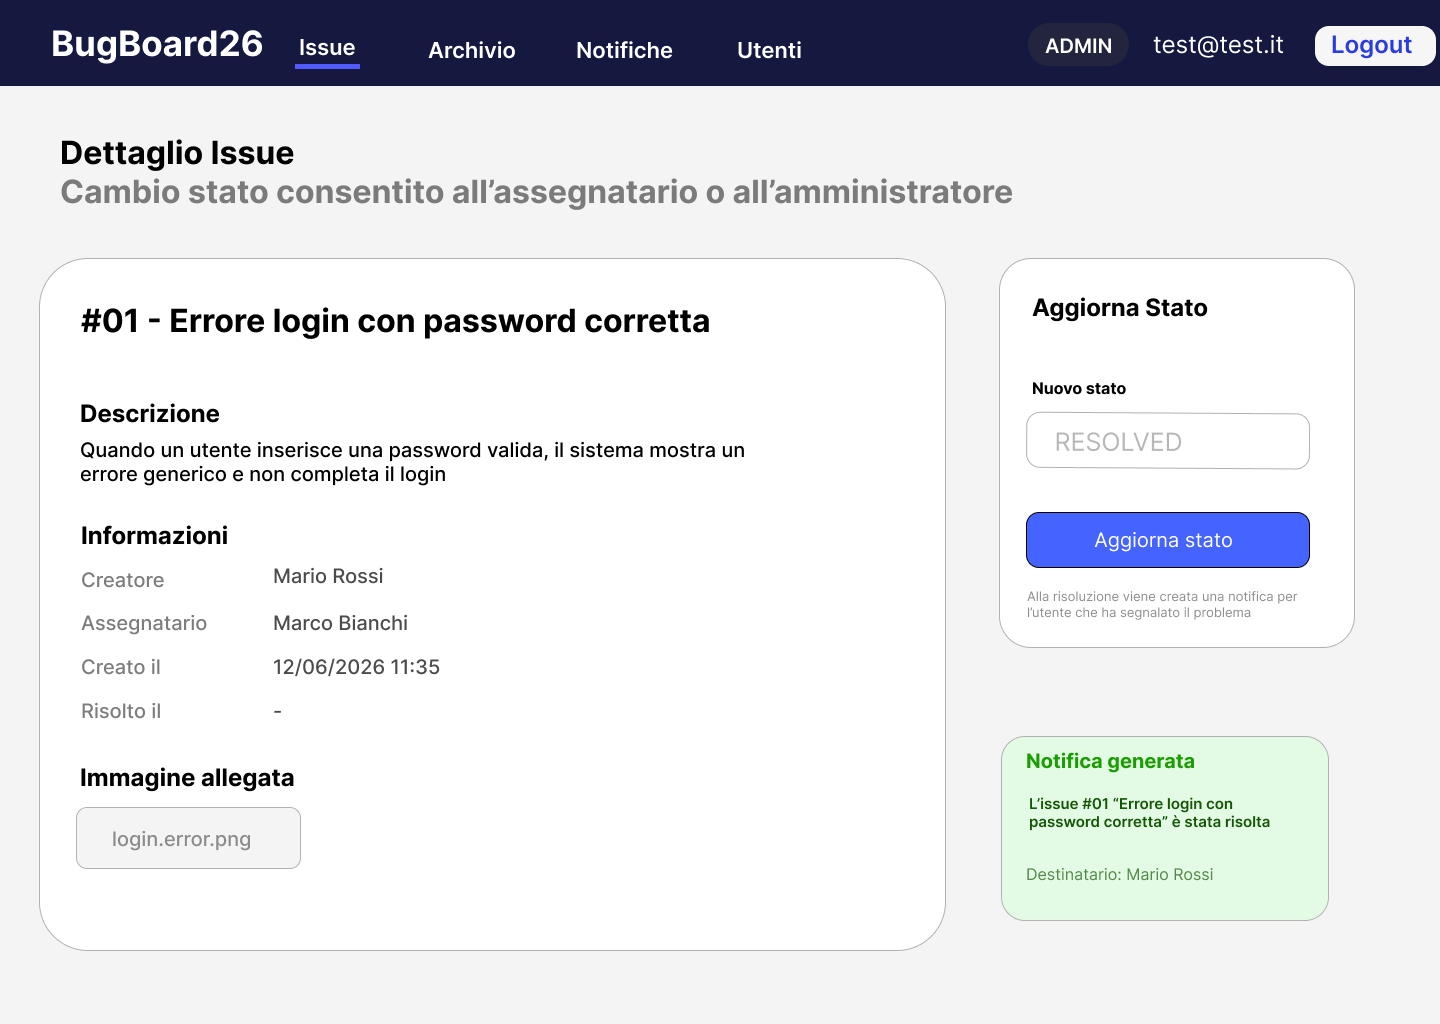
\includegraphics[width=0.9\textwidth]{mock-up/Dettaglio Issue.png}
    \caption{Mock-up - Dettaglio issue e cambio stato}
\end{figure}
}{
\placeholder{Mock-up schermata dettaglio issue}{5cm}
}

\subsection{UC-03 - Contrassegnare una issue come duplicata}

\begin{tabularx}{\textwidth}{>{\bfseries}p{0.28\textwidth} X}
\toprule
Campo & Descrizione \\
\midrule
Attore primario & Amministratore \\
Scopo & Indicare che una issue rappresenta una duplicazione di una issue già esistente. \\
Precondizioni & L'amministratore ha effettuato il login e la issue duplicata esiste nel sistema. \\
Postcondizioni & La issue viene collegata alla issue originale e chiusa con stato \textit{DUPLICATE}. \\
Scenario principale &
\begin{enumerate}[noitemsep]
    \item L'amministratore apre il dettaglio della issue da chiudere come duplicata.
    \item Il sistema mostra l'opzione per contrassegnare la issue come duplicata.
    \item L'amministratore seleziona la issue originale.
    \item Il sistema verifica che la issue originale sia valida.
    \item Il sistema imposta lo stato della issue a \textit{DUPLICATE}.
    \item Il sistema salva il riferimento alla issue originale.
\end{enumerate} \\
Estensioni & Se la issue originale non esiste o coincide con la issue corrente, il sistema rifiuta l'operazione. \\
Requisiti collegati & RF-18, RF-19, RNF-02 \\
\bottomrule
\end{tabularx}

\section{Mock-up previsti}

I mock-up saranno inseriti nella cartella \texttt{mock-up} e usati per descrivere le interazioni principali. In questa fase sono previsti almeno i seguenti:

\begin{itemize}[noitemsep]
    \item schermata di login;
    \item lista issue con ricerca, filtri e ordinamento;
    \item form di creazione issue;
    \item dettaglio issue con cambio stato;
    \item pagina delle issue archiviate;
    \item pagina di gestione utenti per amministratore.
\end{itemize}

\clearpage
\section{Matrice di verifica dei requisiti}

La seguente tabella riassume come si prevede di verificare ogni requisito. La verifica potrà essere svolta tramite test manuali durante la demo, test automatici backend o controllo diretto dell'interfaccia.

\begin{longtable}{>{\bfseries}p{0.12\textwidth} p{0.42\textwidth} p{0.34\textwidth}}
\toprule
ID & Verifica prevista & Esito atteso \\
\midrule
RF-01 & Tentativo di login con credenziali corrette e non corrette. & Con credenziali corrette viene restituito un token; con credenziali errate l'accesso viene negato. \\
RF-02 & Avvio del sistema con database inizializzato. & L'account amministratore di default è presente. \\
RF-03 & Creazione di un utente dalla pagina admin. & Il nuovo utente viene salvato con il ruolo selezionato. \\
RF-04 & Creazione issue con dati validi. & La issue viene creata correttamente. \\
RF-05 & Creazione issue con priorità e immagine opzionali. & I dati opzionali vengono gestiti senza bloccare la creazione. \\
RF-06 & Controllo stato della issue appena creata. & Lo stato iniziale è \textit{TODO}. \\
RF-07 & Accesso alla pagina lista issue. & Sono mostrate le issue non archiviate. \\
RF-08 & Applicazione di filtri e ordinamenti. & La lista cambia coerentemente con i criteri scelti. \\
RF-09 & Ricerca con parola chiave presente in titolo o descrizione. & Sono mostrate solo le issue compatibili con la ricerca. \\
RF-10 & Cambio stato da parte dell'assegnatario e da parte di un utente non autorizzato. & L'assegnatario può modificare; l'utente non autorizzato viene bloccato. \\
RF-11 & Cambio stato a \textit{RESOLVED}. & Il segnalatore riceve una notifica interna. \\
RF-12 & Download dell'export CSV. & Viene prodotto un file CSV leggibile con i dati principali delle issue. \\
RF-13 & Archiviazione da parte di admin. & La issue viene marcata come archiviata. \\
RF-14 & Consultazione lista principale dopo archiviazione. & La issue archiviata non compare nella lista principale. \\
RF-15 & Consultazione pagina archivio. & La issue archiviata è ancora accessibile nella sezione dedicata. \\
RF-16 & Esecuzione algoritmo di suggerimento assegnatario. & Viene suggerito l'utente con minore carico di issue aperte. \\
RF-17 & Tentativo di modifica con utente readonly. & L'utente readonly puo' visualizzare, ma non puo' modificare dati. \\
RF-18 & Contrassegno duplicato da parte di admin. & La issue viene collegata alla issue originale. \\
RF-19 & Controllo stato dopo duplicazione. & La issue duplicata viene chiusa con stato \textit{DUPLICATE}. \\
\bottomrule
\end{longtable}

\section{Requisiti esclusi}

Non sono stati inclusi nel perimetro del progetto i requisiti non assegnati al gruppo, come commenti, etichette personalizzabili, dashboard amministrativa completa, cronologia delle modifiche, report mensili e scadenze. Queste funzionalita' potranno essere considerate come possibili estensioni future, ma non fanno parte della consegna prevista per il gruppo.

\section{Conclusioni}

La specifica definisce una versione di BugBoard26 centrata sulla gestione essenziale delle issue, con attenzione particolare a ruoli, consultazione, ricerca, archiviazione, duplicati e assegnazione. I requisiti sono stati formulati in modo da essere verificabili durante lo sviluppo e durante la discussione finale del progetto.

\end{document}
